\section{Local orbital frame}
\label{sec:local}

\begin{itemize}
    \item[-] \textbf{Give the definition of a geocentric inertial reference frame}

    \textit{Geocentric} refers to the centre of the reference frame being the centre of the Earth. 
    Reference frames can typically be divided into \textit{inertial} and \textit{non-inertial} reference frames, where \textit{inertial} means that the frame is not accelerating (or rotating) and is fixed. 
    The orientation of the coordinate axes is fixed relative to distant stars, typically defined by the vernal equinox and the celestial equator.
    Such frames are more often used due to simplification of the calculation of motion laws.
    
    An example of an often-used geocentric inertial reference frame is the Earth-Centric Inertial (ECI).
    
    \item[-] \textbf{Give the definition of the local orbital frame $R_{LOF}$}
    
    A local orbit reference frame Z-, Y- and X-axis are defined as follows:
    \begin{itemize}
        \item $Z_{ol}$ or \textbf{R}: points directly from the centre of the central body (in this case Earth) towards the orbiting object (in this case the satellite), Zenith direction.
        
        \item $Y_{ol}$ or \textbf{W}: points in the direction of the normal positive to the orbital plane.
    
        \item $X_{ol}$ or \textbf{S}: completes the orthonormal trihedron and in this case points in the direction of the satellite's movement along its orbit.
    \end{itemize} 
    
    \begin{figure}[h]
        \centering
        \subfloat[From lecture slides, (R,S,W) vectors (1-2-3)]
        {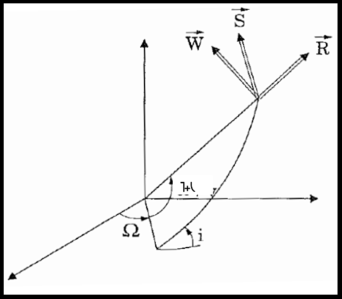
\includegraphics[width=0.4\textwidth]{Graphics/cloe_LOF.png}
        \label{fig:f2-1}}
        %\hfill
        \subfloat[qsw local orbital reference frame]
        {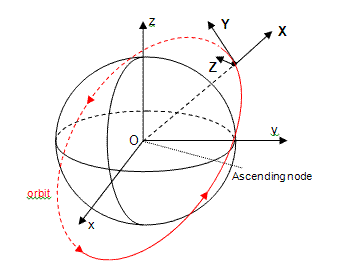
\includegraphics[width=0.45\textwidth]{Graphics/qsw_frame.png}
        \label{fig:f2-2}}
        \caption{The LOF axis can be defined in different ways, such as in (b), where it is the X-axis that follows the radial or zenith direction \cite{ISAE_frames}}
    \end{figure}
    
    
    \newpage
    \item[-] \textbf{Compute the Cubesat local orbital frame vector directions in your geocentric reference frame RE (theoretical computation)}
    

    The transformation matrix for converting LOF to ECI can be found in the lecture slides (1-2-3, slide 49):
    \tiny
    \begin{equation}
    \label{eq:LOF-ECI_transformation_matrix}
    \begin{split}
        &(X, Y, Z)|_{ECI} = (x, y, z)|_{LOF} \cdot \textbf{M}_{\omega + \theta} \cdot \mathbf{M}_{i} \cdot \mathbf{M}_{\Omega} \\
        &= (x, y, z)_{\mathbf{LOF}}
        \begin{bmatrix}
            \cos(\omega + \theta) & \sin(\omega + \theta) & 0 \\
            -\sin(\omega + \theta) & \cos(\omega + \theta) & 0 \\
            0 & 0 & 1
        \end{bmatrix}
        \cdot
        \begin{bmatrix}
            1 & 0 & 0 \\
            0 & \cos(i) & \sin(i) \\
            0 & -\sin(i) & \cos(i)
        \end{bmatrix}
        \cdot
        \begin{bmatrix}
            \cos(\Omega) & \sin(\Omega) & 0 \\
            -\sin(\Omega) & \cos(\Omega) & 0 \\
            0 & 0 & 1
        \end{bmatrix}
    \end{split}
    \end{equation}
    \normalsize

    where:
    \begin{itemize}
       \item $\omega$ is the argument of perigee (40.8630° for the ISS as of Jan 3rd 2025) \cite{ISS_orbit_parameters} 
       \item $\theta$ is the true anomaly (68.2039° for the ISS as of Jan 3rd 2025)   \cite{ISS_orbit_parameters}      
       \item $i$ is the inclination of the orbit (51.6°)
       \item $\Omega$ is the RAAN of the orbit (40.3677° for the ISS as of Jan 3rd 2025) \cite{ISS_orbit_parameters}
    \end{itemize}

    The above transformation matrix can be simplified for calculation by setting $\omega = 0$ and $\theta = 0$, however, this can also be calculated in Python with all values. 
    An example of these vectors is generated in the Python code in \autoref{sec:Appendix_A} on line 94 using the \verb|compute_LOF()| function with the output:
    \begin{lstlisting}[frame=single]
        Transformation Matrix:        
        [[-0.62913233  0.23570859  0.7406983 ]
         [-0.58867996 -0.76675579 -0.25601066]
         [ 0.5075908  -0.59709883  0.62114778]]
        
        Vector in Inertial Frame:
        [ 0.34727457 -1.61144642  0.53163974]
    \end{lstlisting}
    
    \item[-] \textbf{Make a plot of the local orbital frame vector directions (as a function of time)}

    The script for plotting the LOF vector directions can be seen in the Python code in \autoref{sec:Appendix_A} on lines 95 using the \verb|computeandplot_LOF| function.
    \autoref{fig:LOF_plot} shows how the components of the CubeSat's local orbital frame vectors (R, W, S) evolve over time during one orbital period in a circular orbit.

    The R vector points directly from the Earth’s center toward the CubeSat.
    Since the CubeSat orbits in a circular path, the components of R oscillate sinusoidally.     
    The W vector is perpendicular to the orbital plane and for a circular orbit in the equatorial plane, the W vector remains constant along the z-axis.    
    Since the S vector is aligned with the velocity direction, tangent to the orbital path, it also varies sinusoidally, but in a phase shift relative to R since velocity and position are perpendicular.

    \begin{figure}[h]
        \centering
        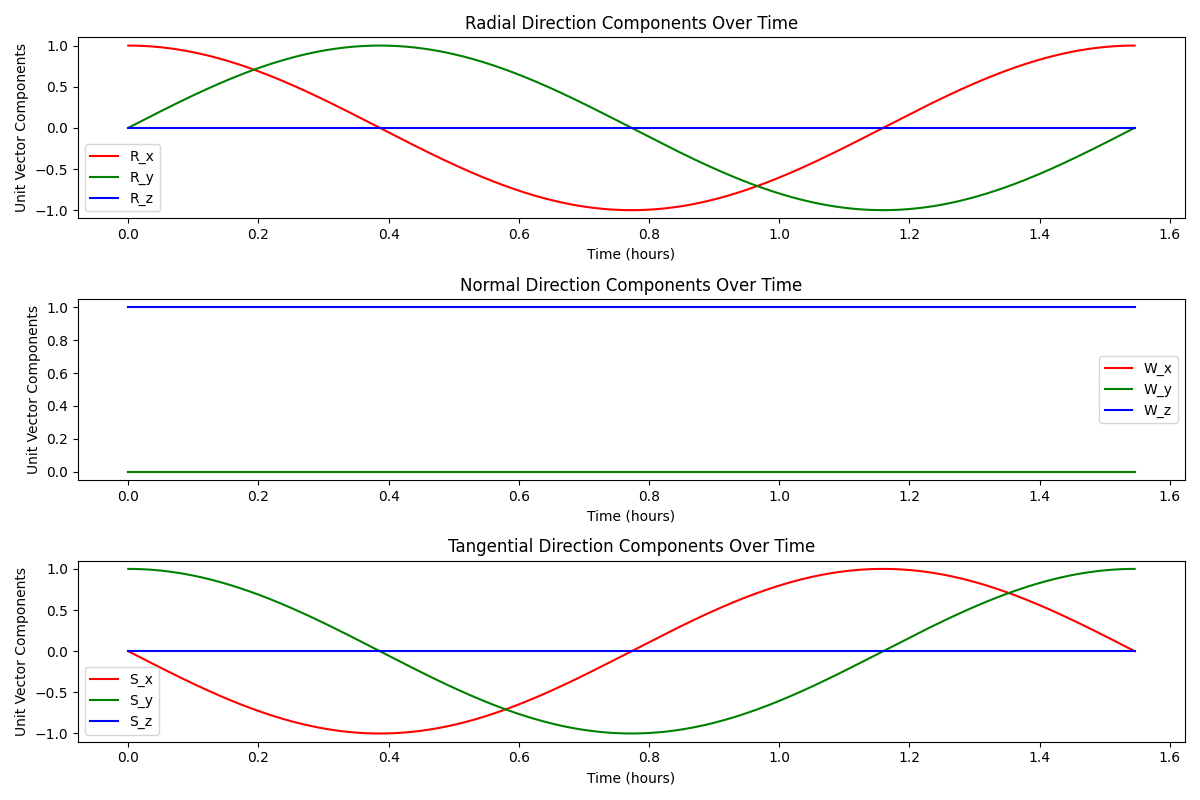
\includegraphics[width=\linewidth]{Doc/Graphics/LOF_vector_directions_plot.png}
        \caption{Plot of LOF vector directions over one orbit}
        \label{fig:LOF_plot}
    \end{figure}
\end{itemize}